% Chapter Template

\chapter{Literature Survey} % Main chapter title

\label{Chapter2} % Change X to a consecutive number; for referencing this chapter elsewhere, use \ref{ChapterX}

\lhead{Chapter 2. \emph{Literature Survey}} % Change X to a consecutive number; this is for the header on each page - perhaps a shortened title

Some of the papers studied for references are:
\begin{itemize}
\item ``Mahnob-HCI-Tagging Database \emph{(Lichtenauer et. al., 2012)}''\cite{mahnobDataset}
\item ``Analysis of EEG signals and facial expressions for continuous emotion detection \emph{(Soleymani et. al., 2015)}''\cite{mahnobEmo}
\item ``Emotion Classification in Arousal Valence Model using MAHNOB-HCI Database \emph{(Wiem et. al., 2017)} \cite''{wiem}
\item ``Selection of the Most Relevant Physiological Features for Classifying Emotion \emph{(Godin et. al., 2015)}''\cite{sel}

After reading these past journals, conference papers and theses, I arrived to these conclusions:
\begin{enumerate}
    \item Human Computer Interaction is a complex topic, and it requires Medical, Mathematical (Signal Processing and Statistical) Knowledge.
    \item There is no way to remove noise and artefacts from collected signal once it has been collected. Hence, while collecting data, you need to be as accurate and careful as possible.
    \item Multiple organs interfere with brain signals and hence are a source of noise to the EEG signals. Subtracting or negating the noise provided by these organs is not always possible, and if possible, it isn't quite precise. Some examples are 
    \begin{enumerate}
        \item Heart activities or ECG signals
        \item Eye Activity, i.e., rotation and focus of the eyes.
        \item Loss of focus or attention by the participant. In this case, the brain activities are not a result of the desired external stimuli , but by wither some internal stimuli or other undesired external stimuli.
    \end{enumerate}
    \item There aren't many clean datasets available freely.
    \item The accuracy varies a lot according to the methodology and dataset used.
    \item Given the brain activity reading, we can segment it into chunks of data of smaller durations, and use the label (ground truth values) on the parent data as the label of all the chunks.
\end{enumerate}
\end{itemize}



% I attempted doing the project using MNE tools in python. I faced quite a bit of issues, and switched to MATLAB for preprocessing.

% Here is the analysis of the signal processing steps, and the reason behind doing the steps:
% \begin{itemize}
% \item Collect High Density EEG Data: The data is collected at a high sampling rate. This is done because data can be down-sampled without loss, however it can't be up-sampled correctly.
% The data collected should be as much free from noise as possible.
% \item The EEG event structure contains records of the experimental events that occurred while the data was being recorded. This can be anything from mouse clicks, video playing on, off, etc.
% \item The data is referenced to either some electrode, or the average reference is taken for each electrode.
% \item The EEG data is down-sampled to reduce the input size. An overwhelming input size may cause over-fitting.
% \item Since the experiment type is Emotion Elicitation, we remove the frequencies which correspond to low activity mental state. Typically, the frequencies below 0.1Hz are removed.
% \item The line noise is removed. Sharp peaks or outliers are smoothed. This is done using a tool called CleanLine.
% \item The required channels are picked and the bad and the channels not required are rejected.
% \item The EEG Epochs corresponding to desired events are chosen.
% \item Finally we run ICA to get the independent components from the electrode signals. ICA finds directions in the feature space corresponding to projections with high non-Gaussianity. We thus obtain a decomposition into independent components, and the artifact’s contribution is localized in only a small number of components. These components have to be correctly identified and removed.
% \end{itemize}

% \section{Difficulties faced}
% \begin{itemize}
% \item Preprocessing the data using MNE python was challenging; there were plenty to methods in the library, but there was no concrete pipeline-based approach to data preprocessing unlike in EEGLab tutorials.
% \item I switched to EEGLab later. However scripting in MATLAB was unfamiliar to me. The way to do the same preprocessing for every EEG file was unknown.
% \item MAHNOB HCI contains 30 seconds of non-event data before and after the actual EEG Signal containing events. Removing these using EEGLAB was difficult as I could find no way to reference index with respect to the end time of the EEG file.
% \item Slicing the EEG data between [30s:-30s] was easy in MNE but data could only be exported as “FIF” file, which was unreadable by EEGLab.
% \end{itemize}

% \section{Experimental Results}
% \begin{itemize}
% \item As of now, I could only process individual EEG file and export the down-sampled, filtered EEG file which contained little noise.
% \item I performed Independent Component Analysis on the data to get the almost uncorrelated dimensions.
% \item I converted the data from time domain to frequency domain and applied PSD to get the four types of Brain Waves : delta, theta, alpha, beta
% \end{itemize}

% \begin{figure}[H]
% \centering
% 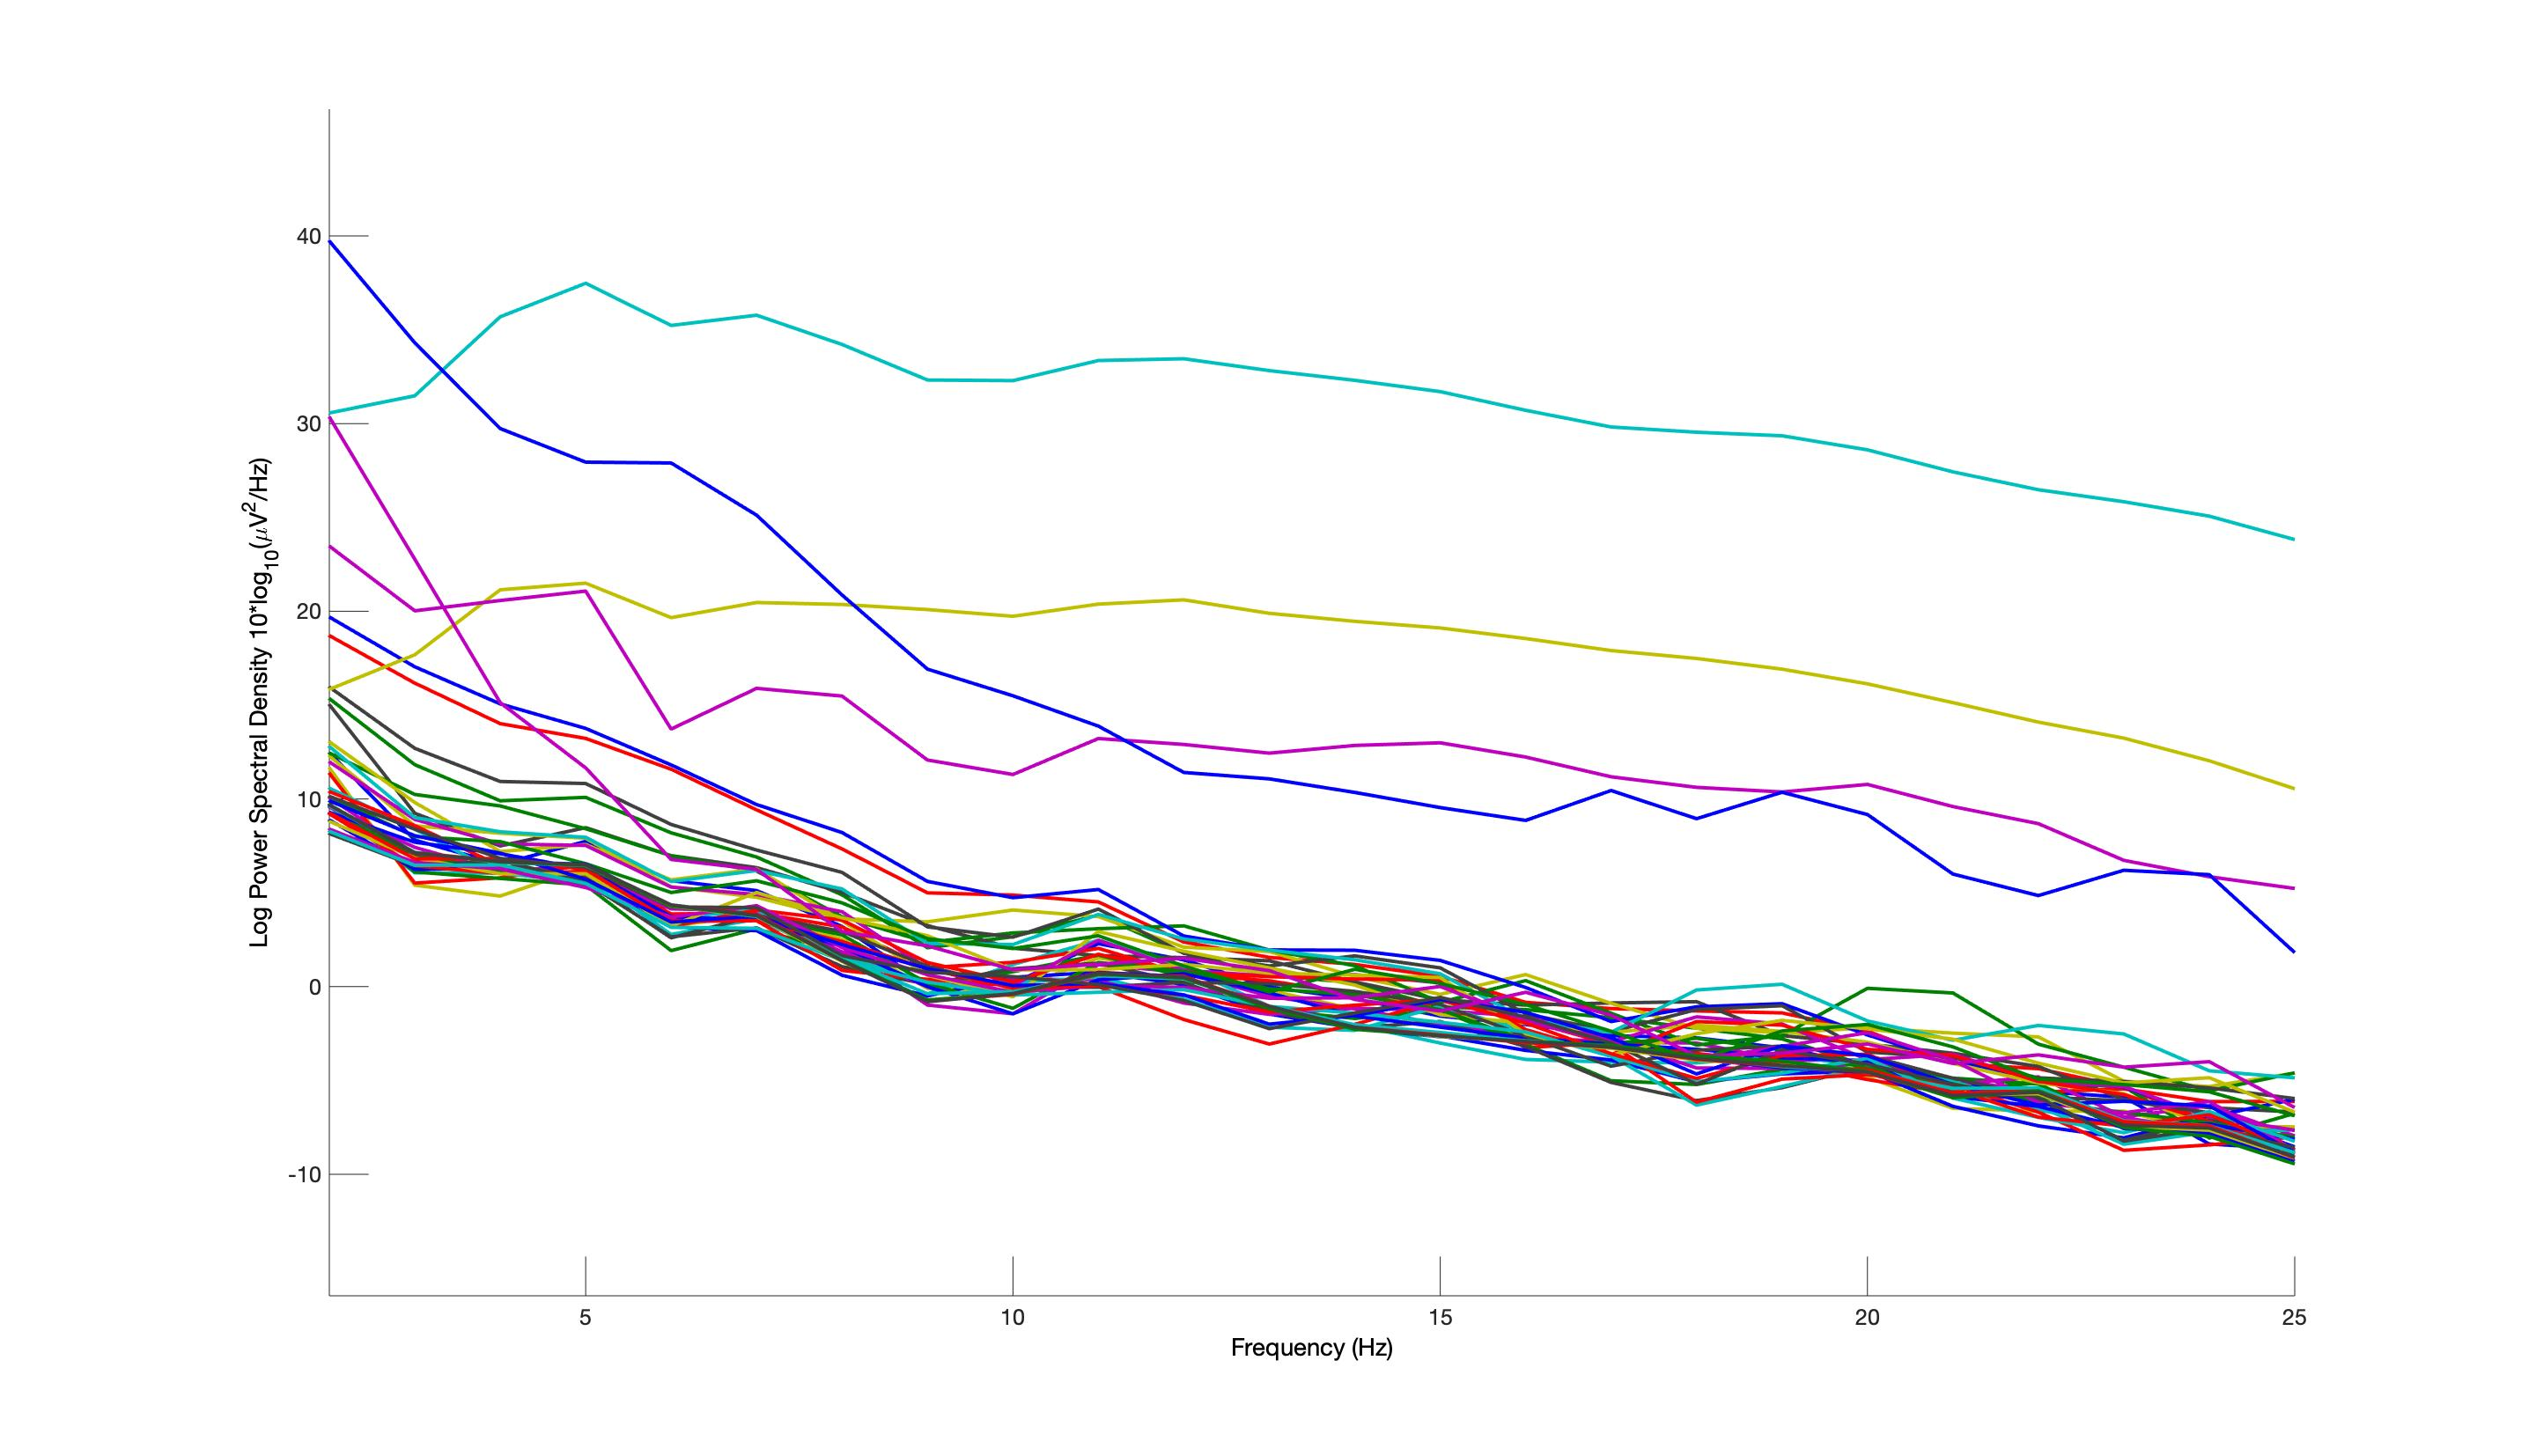
\includegraphics[height=7cm]{Pictures/psd01.jpg}
% \caption{PSD Before Preprocessing}
% \label{fig24}
% \end{figure}
% \begin{figure}[H]
% \centering
% 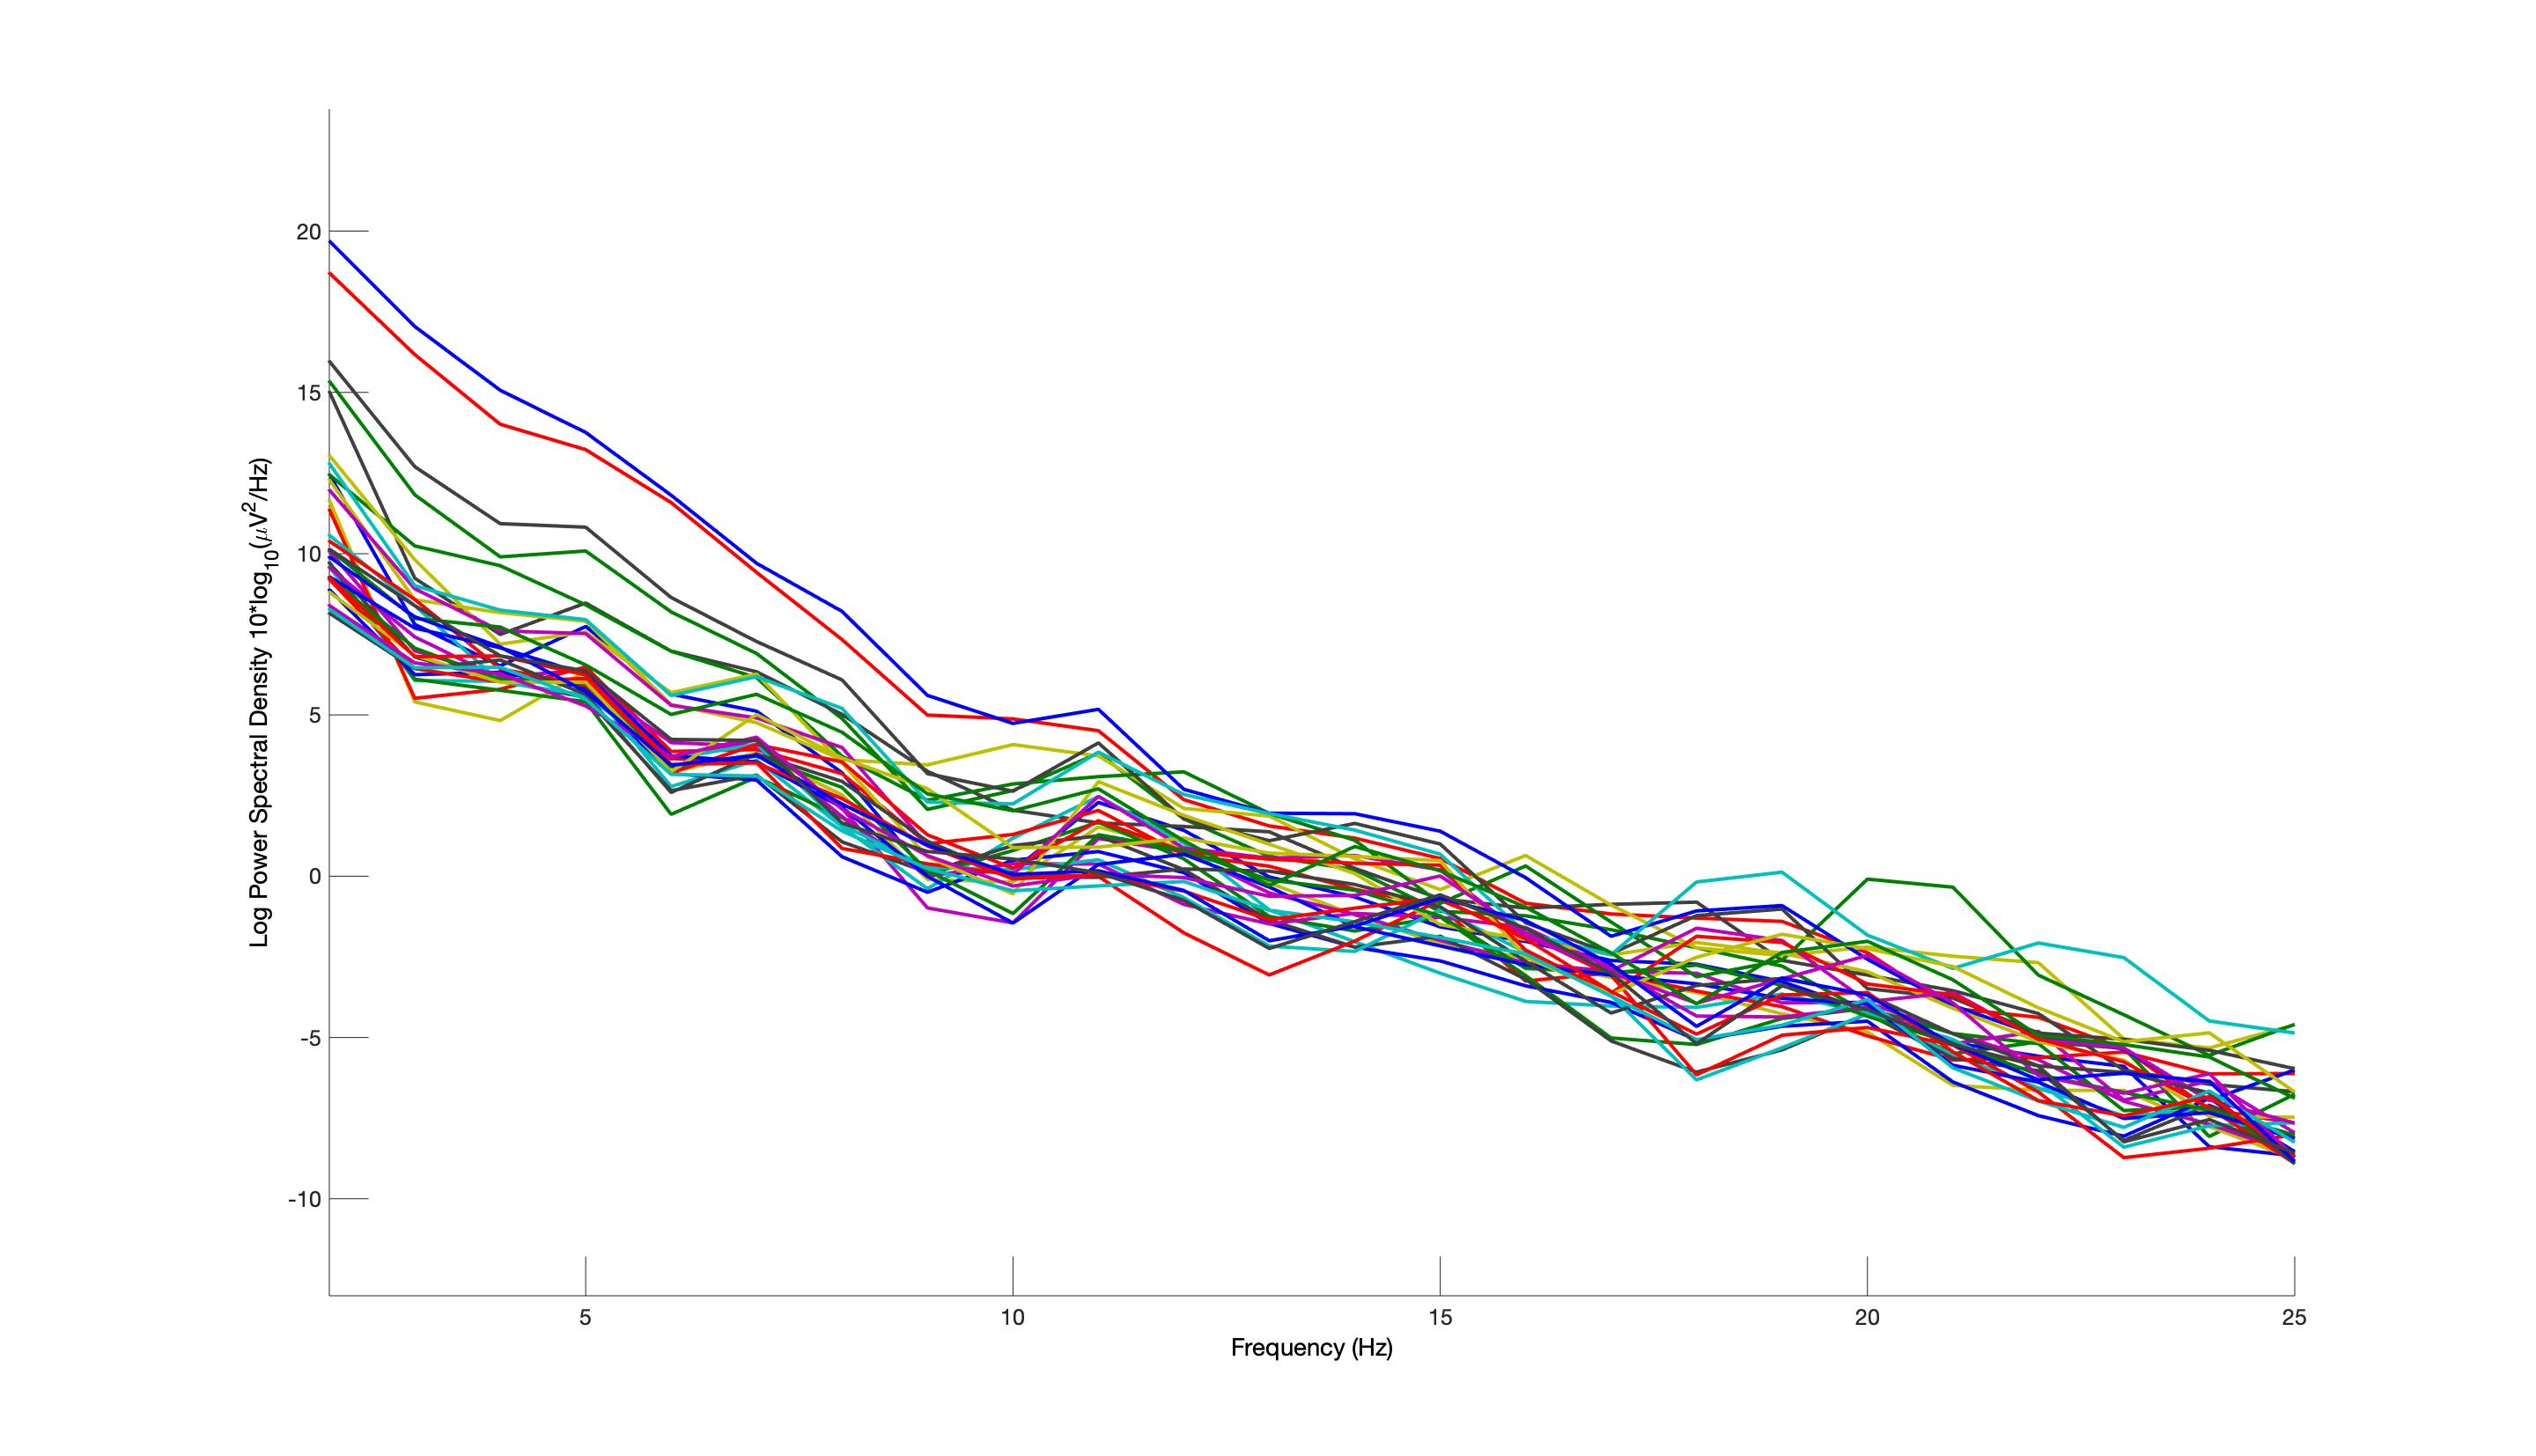
\includegraphics[height=6cm]{Pictures/psd02.jpg}
% \caption{PSD After Preprocessing}
% \label{fig25}
% \end{figure}

% \begin{figure}[H]
% \centering
% 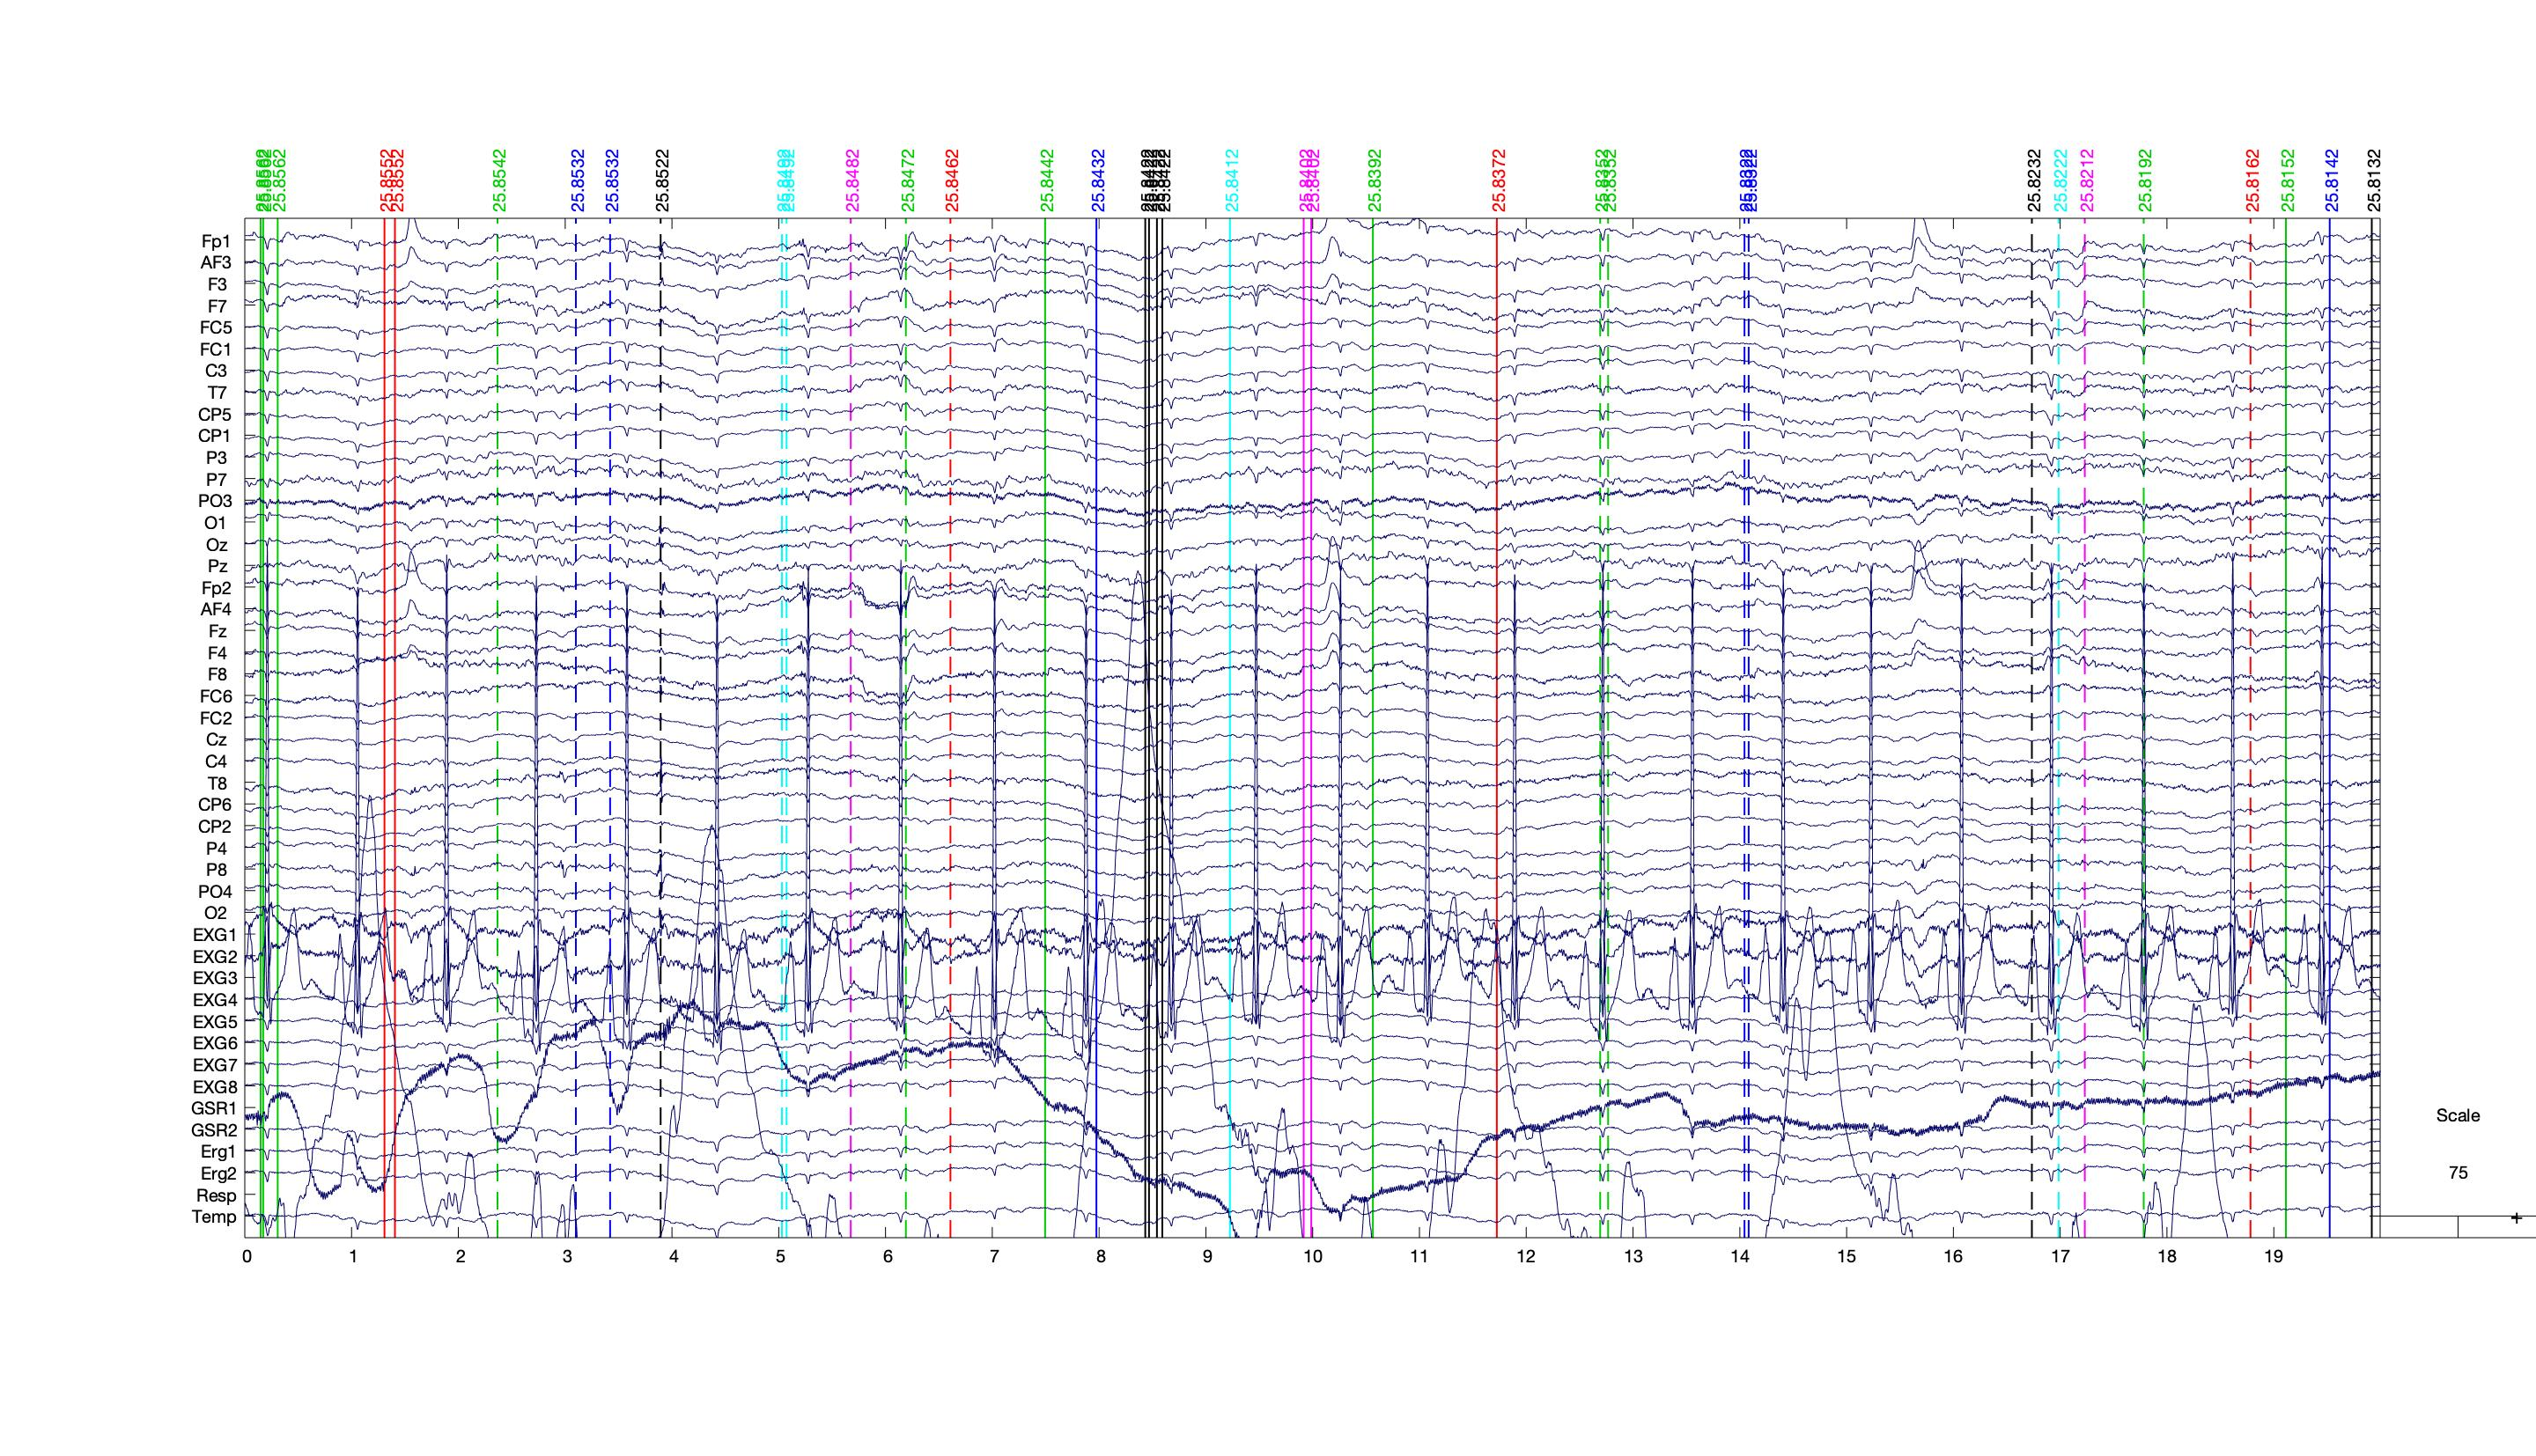
\includegraphics[height=6cm]{Pictures/tm02.jpg}
% \caption{Amplitude vs Time Before Preprocessing}
% \label{fig26}
% \end{figure}
% \begin{figure}[H]
% \centering
% 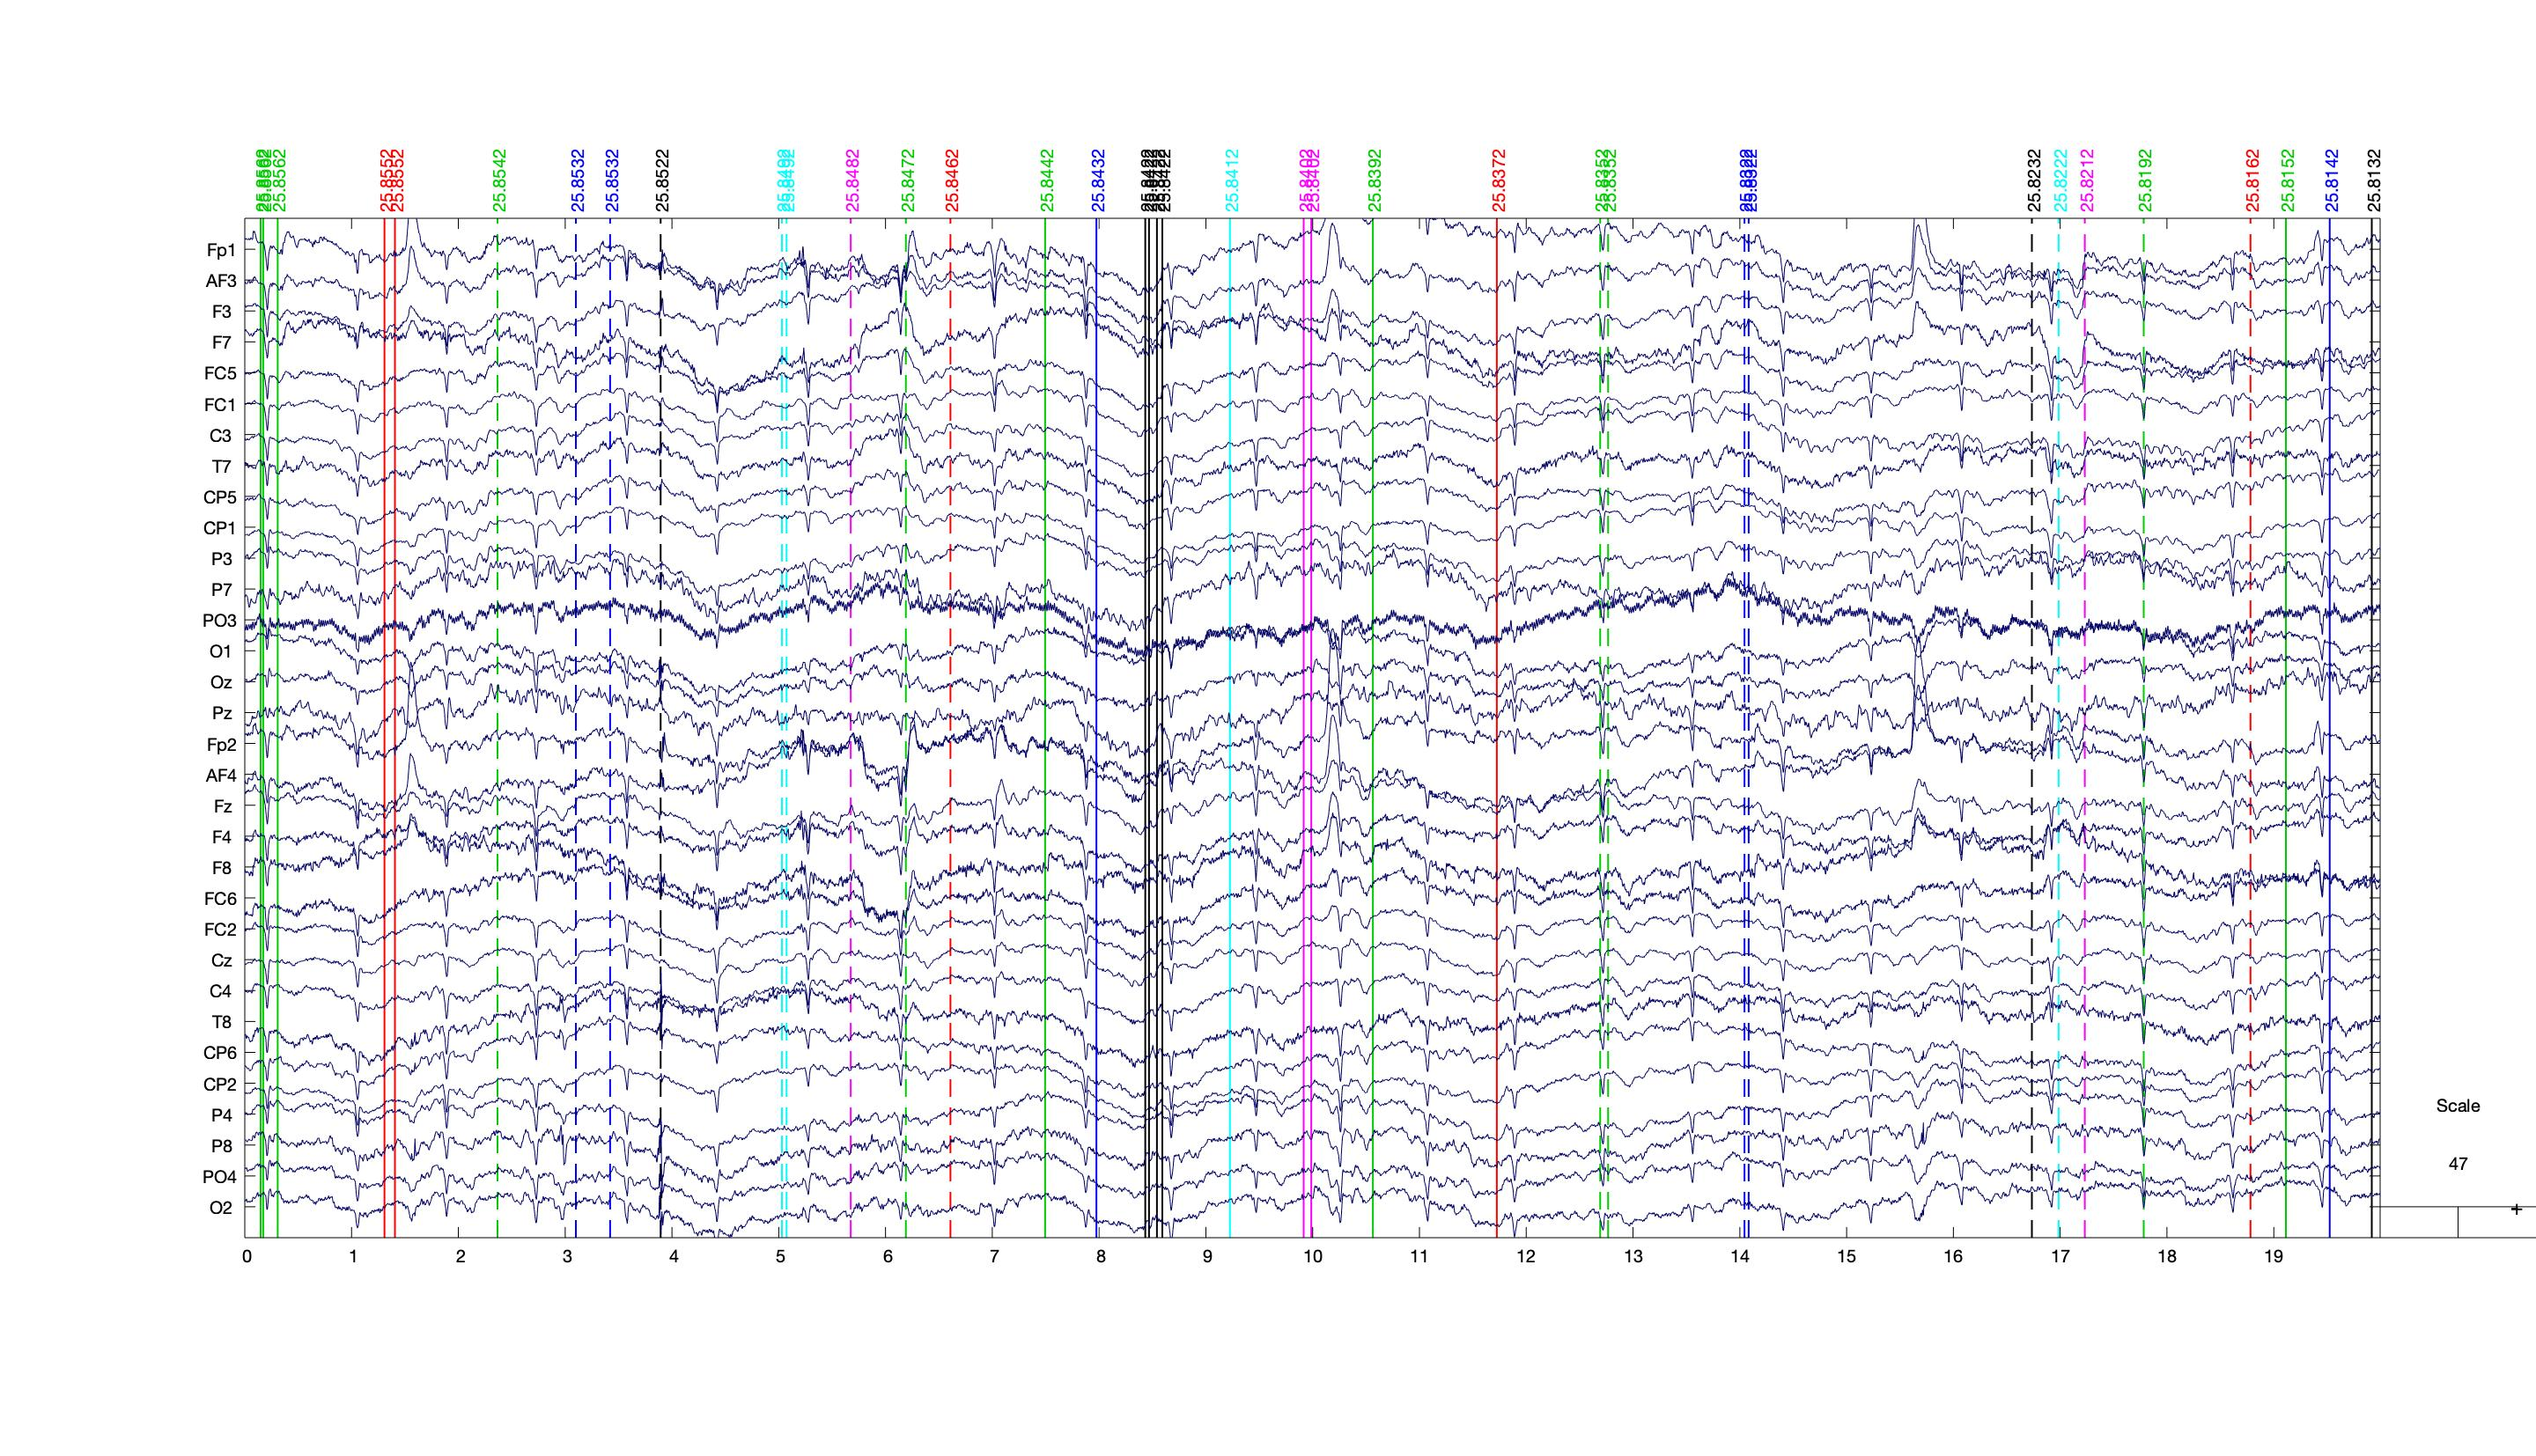
\includegraphics[height=6cm]{Pictures/tm01.jpg}
% \caption{Amplitude vs Time After Preprocessing}
% \label{fig27}
% \end{figure}

% \section{Future Work}
% In the future, exploring novel methods of feature extraction and fitting these into classifying models such as regression models, SVM, XGBoost etc. will be the focus. I also plan to trying out analysis and experiments in Python, because being a veteran programming language, projects and code in python can easily be extended and reproduced.
